\phantomsection\addcontentsline{toc}{section}{BS in CS Class Schedule}%
\label{plan:bs-cs}%
\section*{Bachelor of Science: Computer Science}
\begin{center}
Suggested Class Schedule for Computer Science and Math Courses.
% \def\svgwidth{0.9\textwidth}
% \input{./images/PrerequisiteDiagram_BS_ComputerScience.pdf_tex}

% 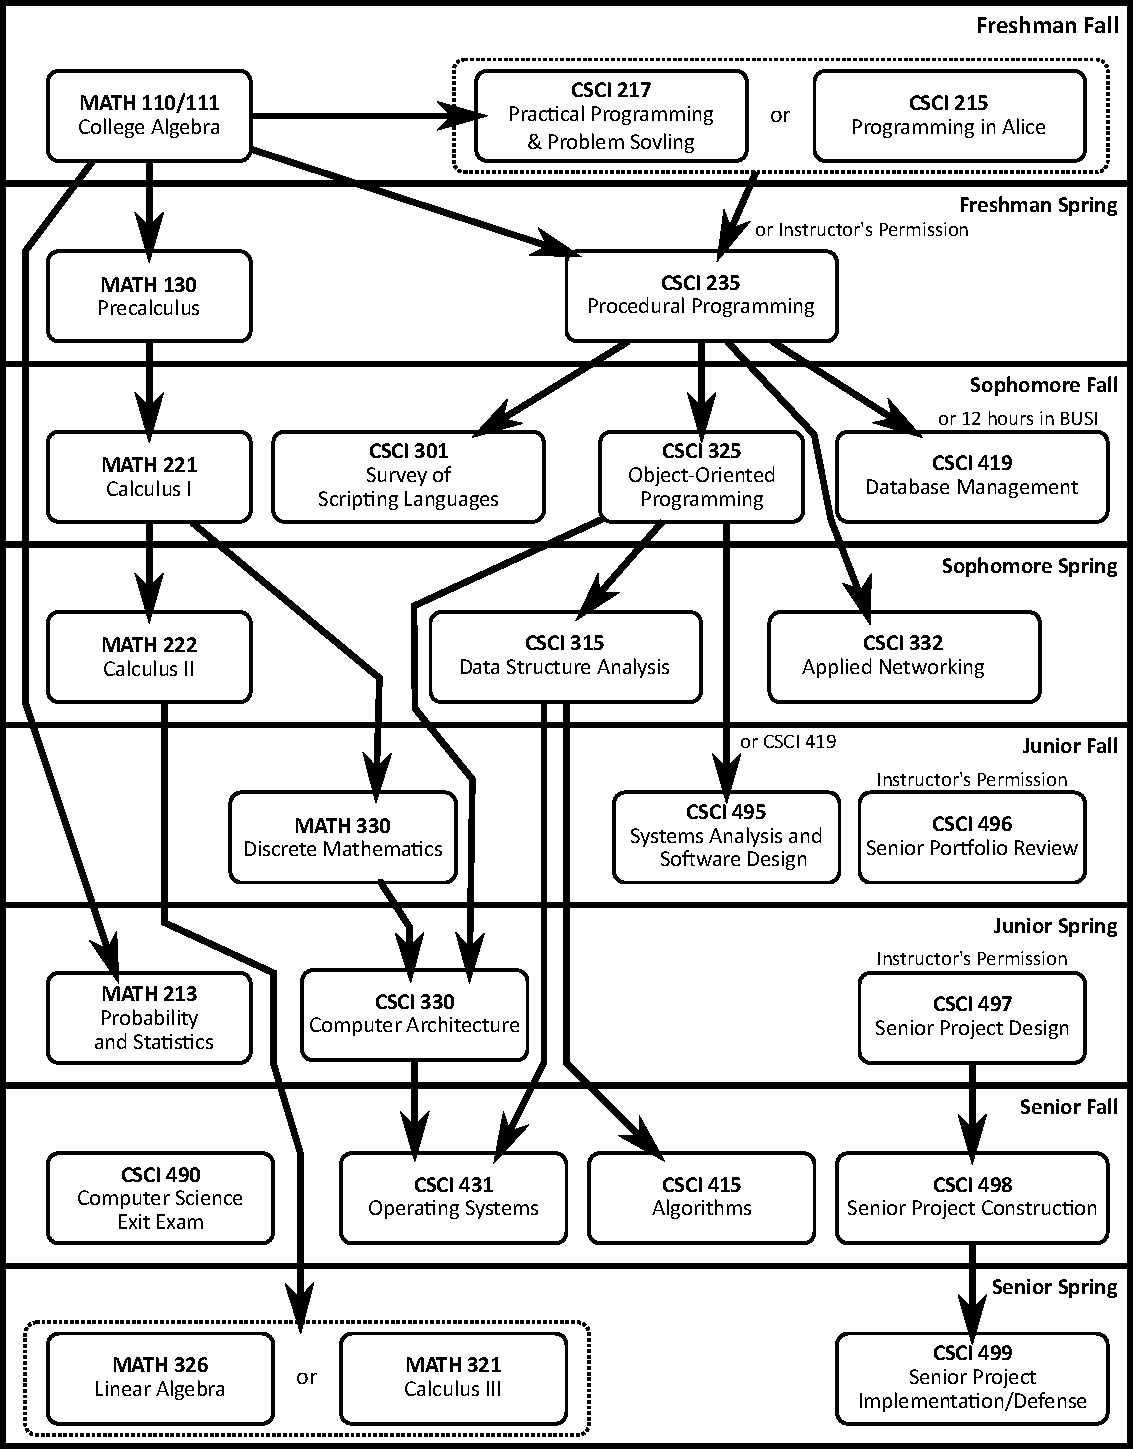
\includegraphics[width=0.86\textwidth]{images/PrerequisiteDiagram_BS_ComputerScience}


\begin{tikzpicture}[x=1cm,y=1cm]
  \draw[black,line width=1pt,rounded corners=4pt] (-1,1.5) rectangle (18,-18.5);

  % ===== Semester labels and separators =====
  \semester{0}{Freshman Fall}
  \semester{1}{Freshman Spring}
  \semester{2}{Sophomore Fall}
  \semester{3}{Sophomore Spring}
  \semester{4}{Junior Fall}
  \semester{5}{Junior Spring}
  \semester{6}{Senior Fall}
  \semester{7}{Senior Spring}
  \foreach \i in {0,...,6}{\rowrule{\i}}

  % ===== Course catalog and placement =====
  \course{math110}{1.25}{0}{MATH 110/111}{College Algebra}
  \course{csci217}{7}{0}{CSCI 217}{Practical Programming\\\& Problem Solving}
  \course{csci215}{11}{0}{CSCI 215}{Programming in Alice}

  \course{math130}{1.25}{1}{MATH 130}{Precalculus}
  \course{csci235}{9}{1}{CSCI 235}{Procedural Programming}

  \course{math221}{1.25}{2}{MATH 221}{Calculus I}
  \course{csci301}{5.25}{2}{CSCI 301}{Survey of\\Scripting Languages}
  \course{csci325}{9}{2}{CSCI 325}{Object-Oriented\\Programming}
  \course{csci419}{13}{2}{CSCI 419}{Database Management}

  \course{math222}{1.25}{3}{MATH 222}{Calculus II}
  \course{csci315}{9}{3}{CSCI 315}{Data Structure Analysis}
  \course{csci332}{13}{3}{CSCI 332}{Applied Networking}

  \course{math330}{5.25}{4}{MATH 330}{Discrete Mathematics}
  \course{csci495}{11}{4}{CSCI 495}{Systems Analysis and\\Software Design}
  \course{csci496}{14.75}{4}{CSCI 496}{Senior Portfolio Review}

  \course{math213}{1.25}{5}{MATH 213}{Probability\\and Statistics}
  \course{csci330}{5.25}{5}{CSCI 330}{Computer Architecture}
  \course{csci497}{14.75}{5}{CSCI 497}{Senior Project Design}

  \course{csci490}{1.25}{6}{CSCI 490}{Computer Science\\Exit Exam}
  \course{csci431}{5.25}{6}{CSCI 431}{Operating Systems}
  \course{csci415}{9}{6}{CSCI 415}{Algorithms}
  \course{csci498}{14.75}{6}{CSCI 498}{Senior Project\\Construction}

  \course{math326}{1.25}{7}{MATH 326}{Linear Algebra}
  \course{math321}{5.25}{7}{MATH 321}{Calculus III}
  \course{csci499}{14.75}{7}{CSCI 499}{Senior Project\\Implementation/Defense}

  % ===== Alternative course groupings =====
  \node[alternative,fit=(csci217)(csci215)] (introchoice) {};
  \node[note] at ($(csci217.east)!.5!(csci215.west)$) {or};
  \node[alternative,fit=(math326)(math321)] (mathchoice) {};
  \node[note] at ($(math326.east)!.5!(math321.west)$) {or};

  % ===== Prerequisite edges (edit independently of courses) =====
  \prereq{math110}{csci235}
  \prereq{math110}{math130}
  \prereq{math130}{math221}
  \prereq{math221}{math222}
  \prereq{math330}{csci330}
  \prereq{csci235}{csci325}
  \prereq{csci235}{csci301}
  % \prereq{csci235}{csci419}
  \prereq{csci325}{csci315}
  % \prereq{csci325}{csci495}
  \prereq{csci330}{csci431}
  \prereq{csci497}{csci498}
  \prereq{csci498}{csci499}
  \prereq{csci315}{csci415}

  % Additional connections, using intermediate coordinates for clean routing.
  \draw[prerequisite] (math110.east) -- (csci217.west);
  \draw[prerequisite] (introchoice) -- (csci235) node[pos=1,note,anchor=south west,xshift=0.25em] {or Instructor's Permission};
  \draw[prerequisite] (csci235) -- (csci419) node[pos=1,note,anchor=south west,xshift=0.25em] {or 12 hours in BUSI};

  % Vertical lanes (x only) that long routes travel down between course columns.
  \coordinate (laneNetwork) at ($(csci325.east)!.5!(csci419.west)$);
  \coordinate (laneMath) at ($(math213.east)!.5!(math330.west)$);
  \coordinate (laneDiscrete) at ($(math330.east)!.5!(csci315.west)$);
  \coordinate (laneWest) at ($(math130.west)+(-2.5mm,0)$);
  \coordinate (laneDiscreteEast) at ($(math330.east)+(+5mm,0)$);

  \longroute{csci235}{0.5}{laneNetwork}{csci332}
  \longroute{csci325}{0.5}{laneNetwork}{csci495}
  \longroute{csci315}{-0.5}{laneDiscreteEast}{csci431}
  \longroute{math221}{0.75}{laneMath}{math330}
  \longroute{math222}{0}{laneMath}{mathchoice}
  \longroute{math110}{-0.9}{laneWest}{math213}
  \longroute{csci325}{-0.75}{laneDiscrete}{csci330}
  \node[note,anchor=south west,xshift=0.25em] at (csci495.north) {or CSCI 419};
  \node[note,anchor=south, yshift=0.1pt] at (csci496.north) {Instructor's Permission};
  \node[note,anchor=south, yshift=0.1pt] at (csci497.north) {Instructor's Permission};
\end{tikzpicture}
\end{center}